\startappendix{Appendix}
\label{chapter: Additional Models}



\section{Stream Data plots}

\begin{figure}[H]
\centering
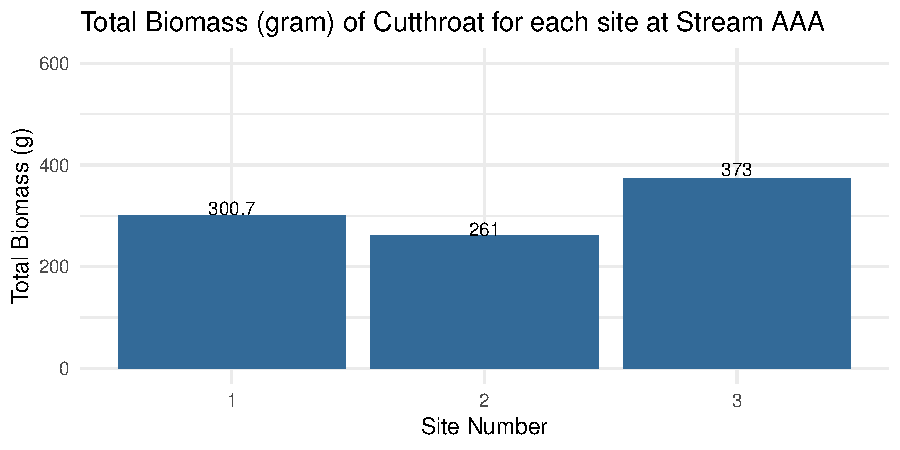
\includegraphics{AppendixImages/AAA_Ct_new.pdf}
\caption{\hspace{1mm}     Total Biomass of Cutthrout Trout at Stream AAA.}
\label{fig:testAAAbiom}
\end{figure}


\begin{figure}[H]
\centering
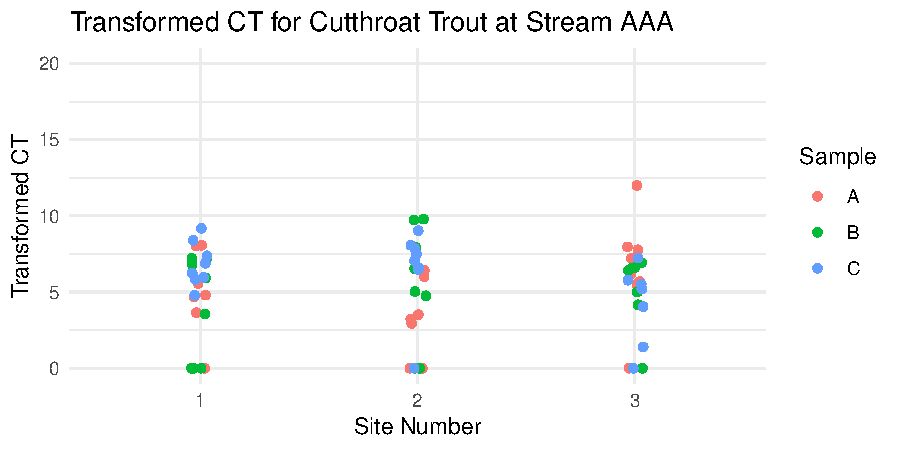
\includegraphics{AppendixImages/AAA_ct_tct.pdf}
\caption{  \hspace{1mm}   Transformed CT values taken over technical replicates for Cutthroat Trout.}
\label{fig:AAA_ct}
\end{figure}




\begin{figure}[H]
\centering
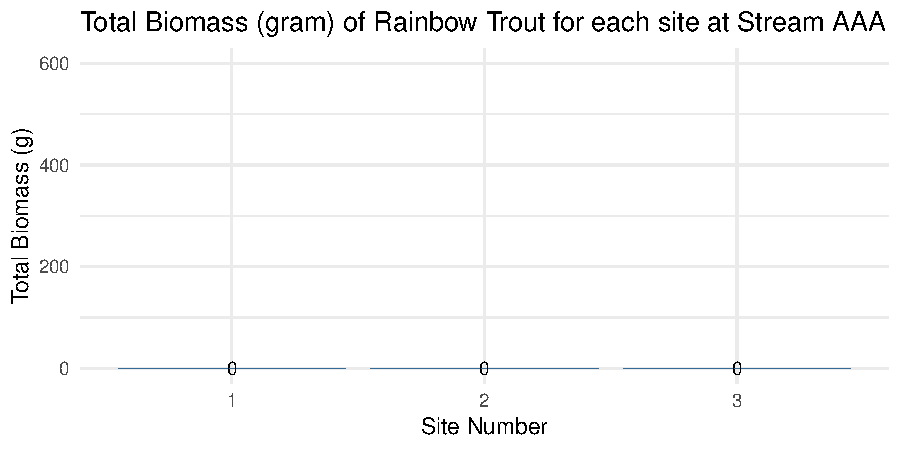
\includegraphics{AppendixImages/AAA_Rb_new.pdf}
\caption{\hspace{1mm}   Total Biomass for Rainbow Trout at Stream AAA.}
\label{fig:AAA_rb_new}
\end{figure}



\begin{figure}[H]
\centering
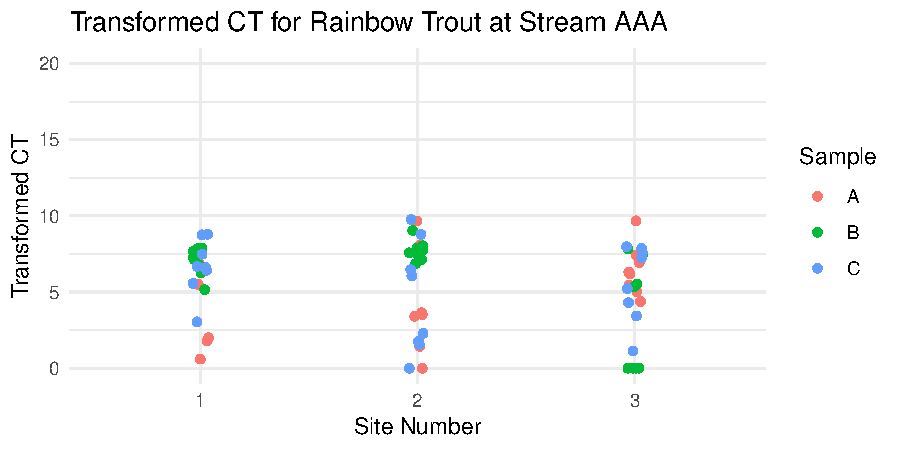
\includegraphics{AppendixImages/AAA_rb_tct.pdf}
\caption{ \hspace{1mm}    Transformed CT values taken over technical replicates for Rainbow Trout.}
\label{fig:AAA_rb}
\end{figure}





\begin{figure}[H]
\centering
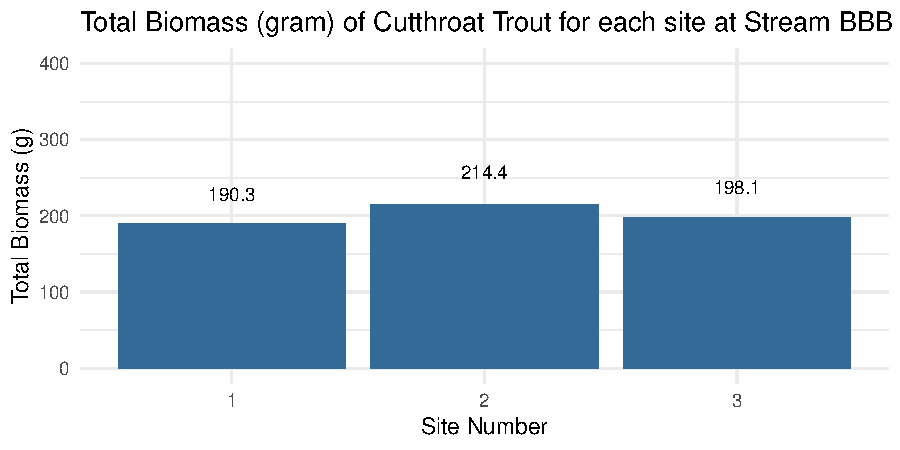
\includegraphics{AppendixImages/BBB_Ct_new.pdf}
\caption{ \hspace{1mm}    Total biomass for Cutthroat Trout at each site for Stream BBB.}
\label{fig:testBBBbiom2}
\end{figure}





\begin{figure}[H]
\centering
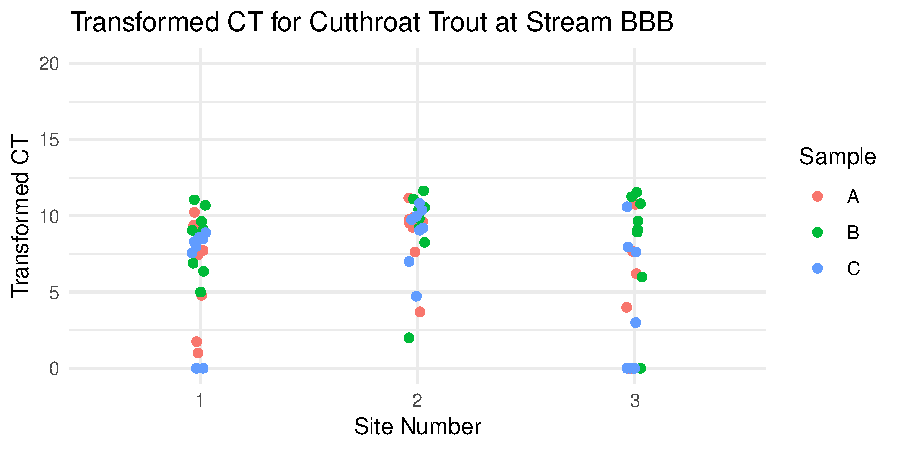
\includegraphics{AppendixImages/BBB_ct_tct.pdf}
\caption{  \hspace{1mm}  Transformed CT values taken over technical replicates for Cutthroat Trout.}
\label{fig:BBB_ct}
\end{figure}




\begin{figure}[H]
\centering
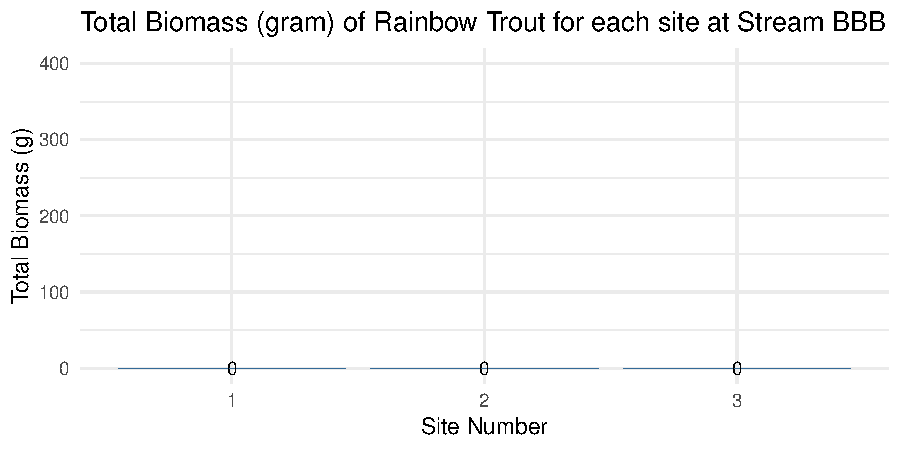
\includegraphics{AppendixImages/BBB_Rb_new.pdf}
\caption{  \hspace{1mm}  Total biomass for Rainbow Trout at each site for Stream BBB.}
\label{fig:testBBBbiomRb}
\end{figure}




\begin{figure}[H]
\centering
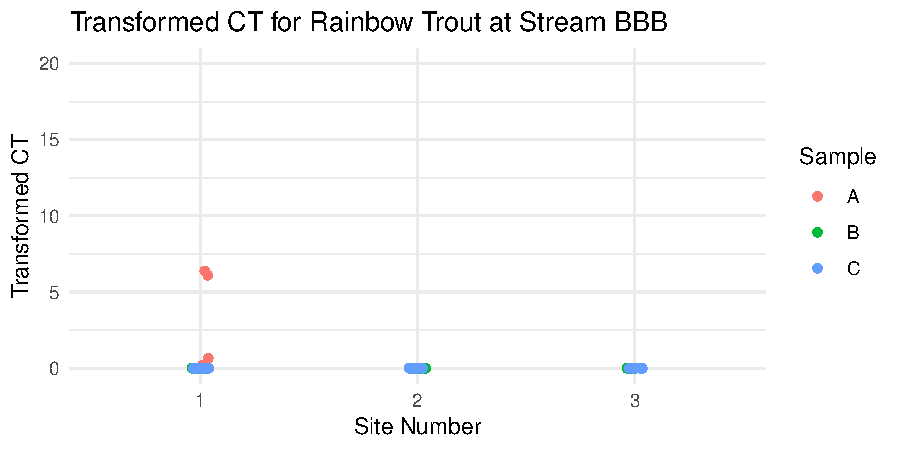
\includegraphics{AppendixImages/BBB_rb_tct.pdf}
\caption{ \hspace{1mm}  Transformed CT values taken over technical replicates for Rainbow Trout.}
\label{fig:BBB_rb}
\end{figure}







\begin{figure}[H]
\centering
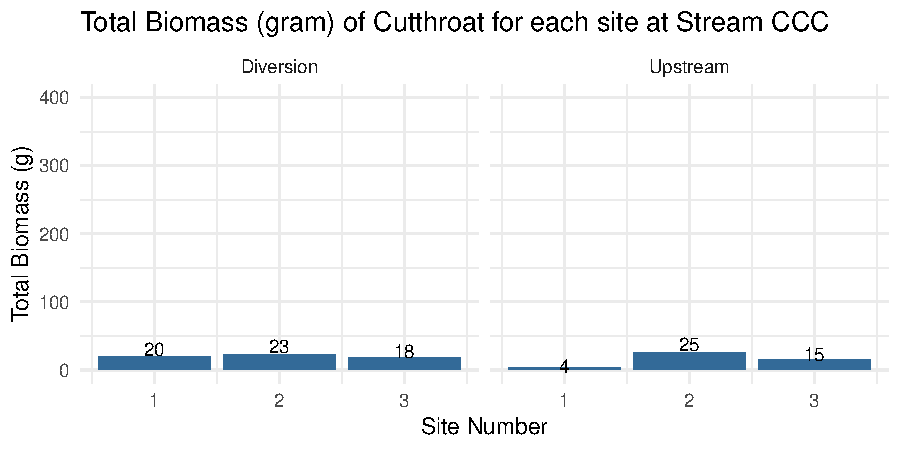
\includegraphics{AppendixImages/CCC_Ct_new.pdf}
\caption{  \hspace{1mm}   Total biomass for Cutthroat Trout at each site for Stream CCC.}
\label{fig:testCCCbiomCt}
\end{figure}





\begin{figure}[H]
\centering
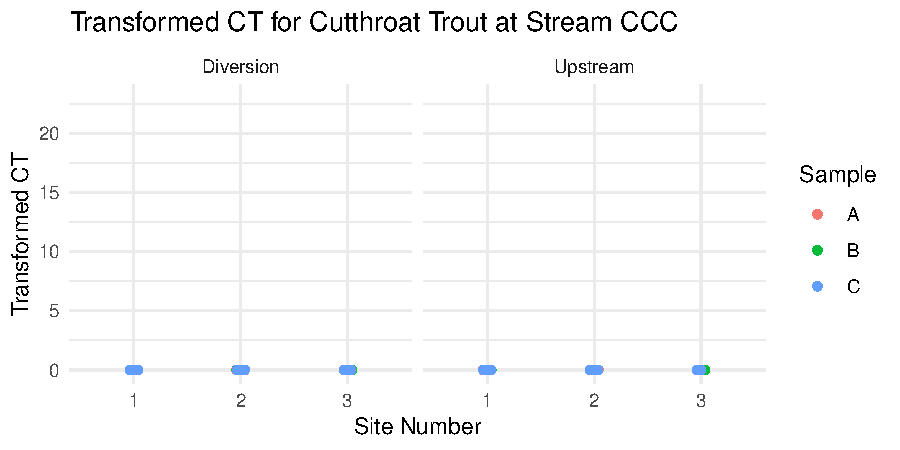
\includegraphics{AppendixImages/CCC_ct_tct.pdf}
\caption{ \hspace{1mm}    Transformed CT values taken over technical replicates for Cutthroat Trout.}
\label{fig:CCC_ct}
\end{figure}




\begin{figure}[H]
\centering
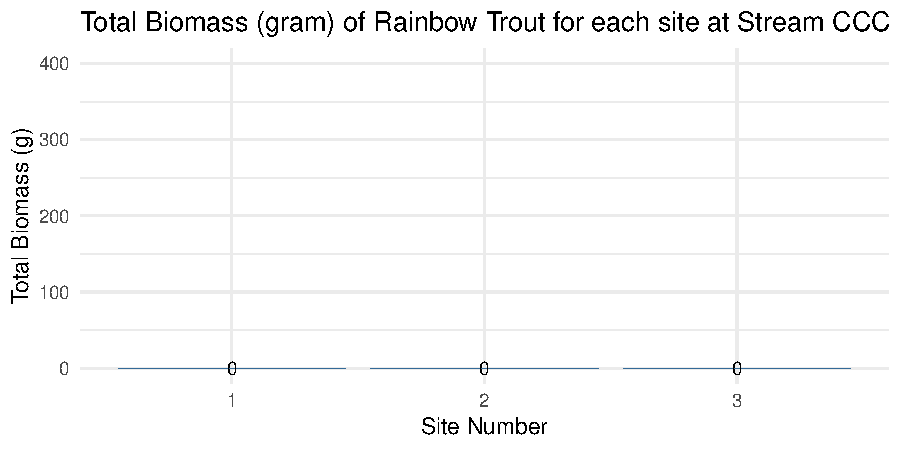
\includegraphics{AppendixImages/CCC_Rb_new.pdf}
\caption{  \hspace{1mm}   Total biomass for Rainbow Trout at each site for Stream CCC.}
\label{fig:testCCCbiomRb}
\end{figure}





\begin{figure}[H]
\centering
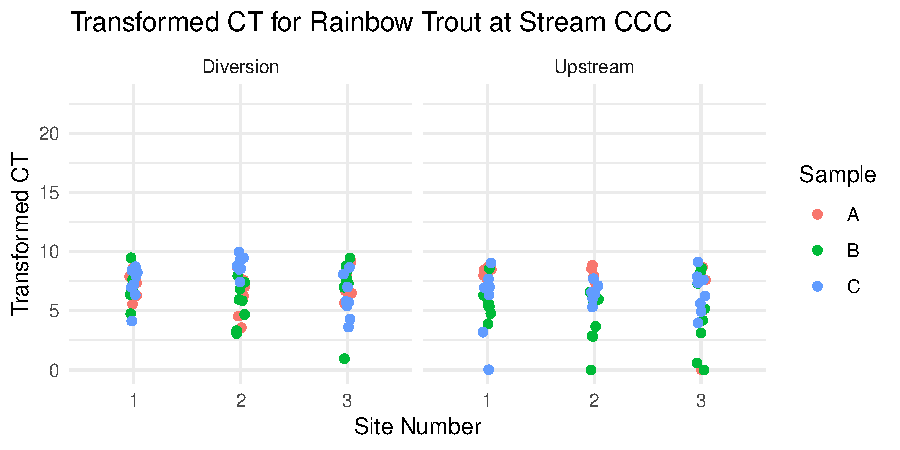
\includegraphics{AppendixImages/CCC_rb_tct.pdf}
\caption{  \hspace{1mm}   Transformed CT values taken over technical replicates for Rainbow Trout.}
\label{fig:CCC_rb}
\end{figure}



\begin{figure}[H]
\centering
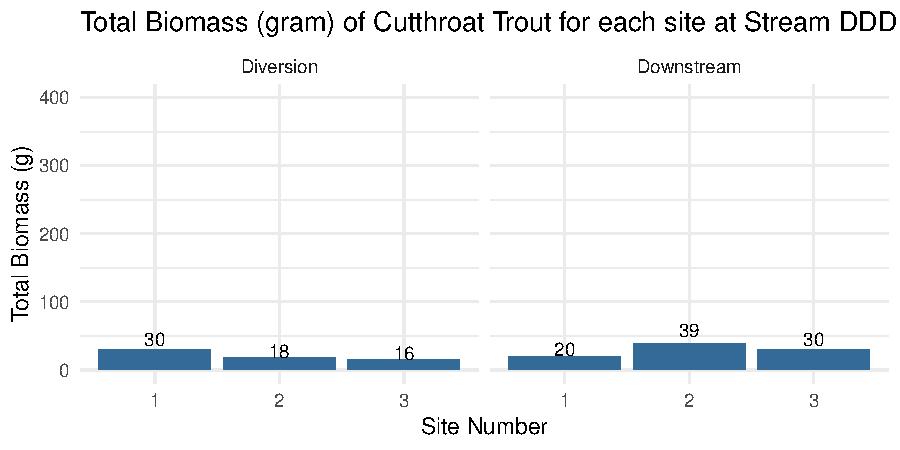
\includegraphics{AppendixImages/DDD_Ct_new.pdf}
\caption{ \hspace{1mm}    Total biomass for Cutthroat Trout at each site for Stream DDD.}
\label{fig:testDDDCt}
\end{figure}



\begin{figure}[H]
\centering
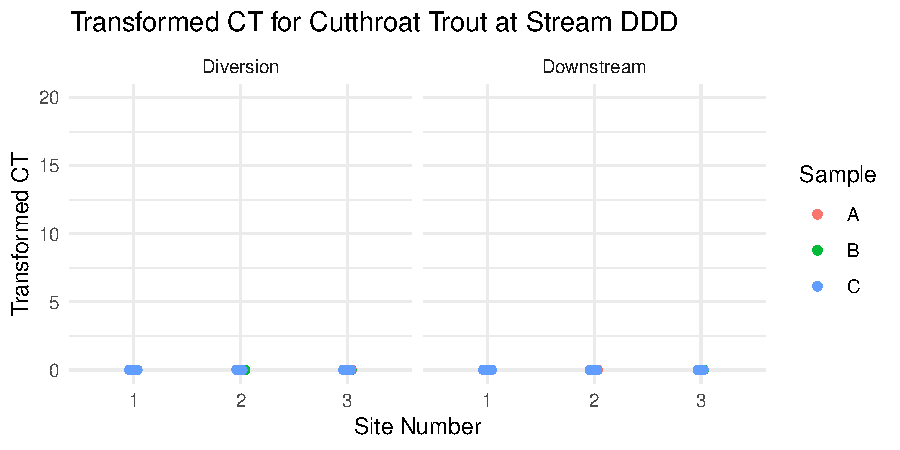
\includegraphics{AppendixImages/DDD_ct_tct.pdf}
\caption{  \hspace{3mm}   Transformed CT values taken over technical replicates for Cutthroat Trout.}
\label{fig:DDD_ct}
\end{figure}


\begin{figure}[H]
\centering
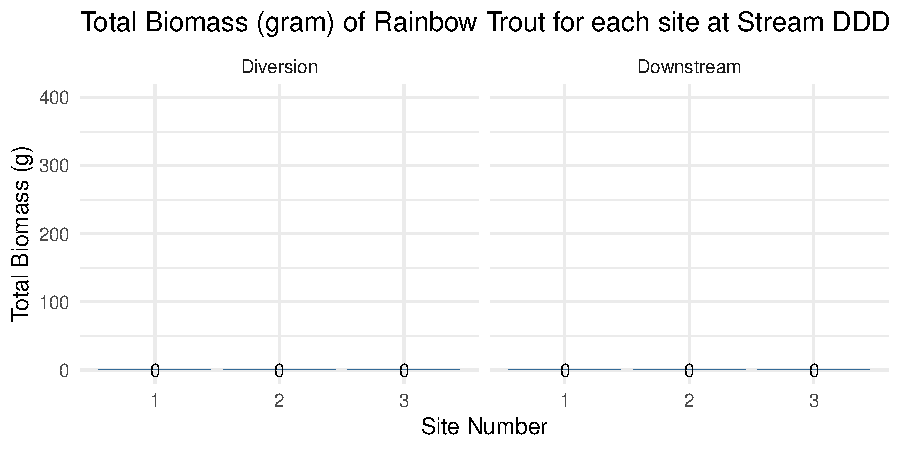
\includegraphics{AppendixImages/DDD_Rb_new.pdf}
\caption{ \hspace{1mm}    Total biomass for Rainbow Trout at each site for Stream DDD.}
\label{fig:testDDDrb}
\end{figure}




\begin{figure}[H]
\centering
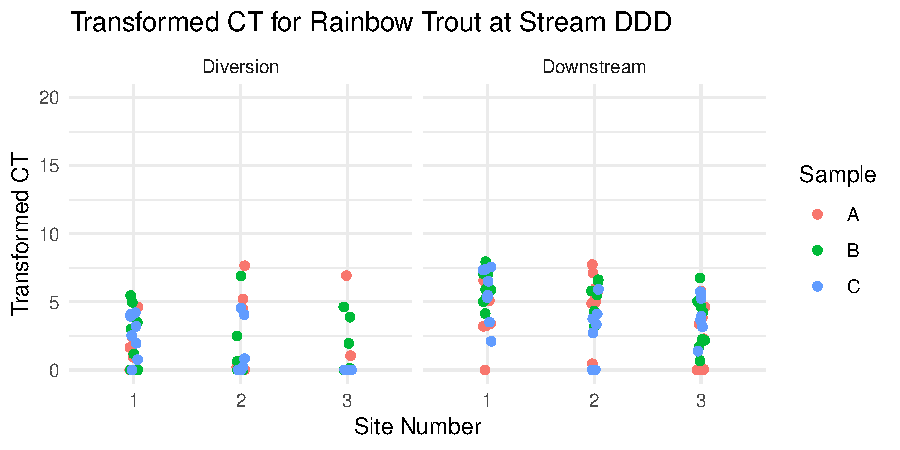
\includegraphics{AppendixImages/DDD_rb_tct.pdf}
\caption{ \hspace{1mm}  Transformed CT values taken over technical replicates for Rainbow Trout.}
\label{fig:DDD_rb}
\end{figure}




\section{Pairs Plots}

\begin{figure}[H]
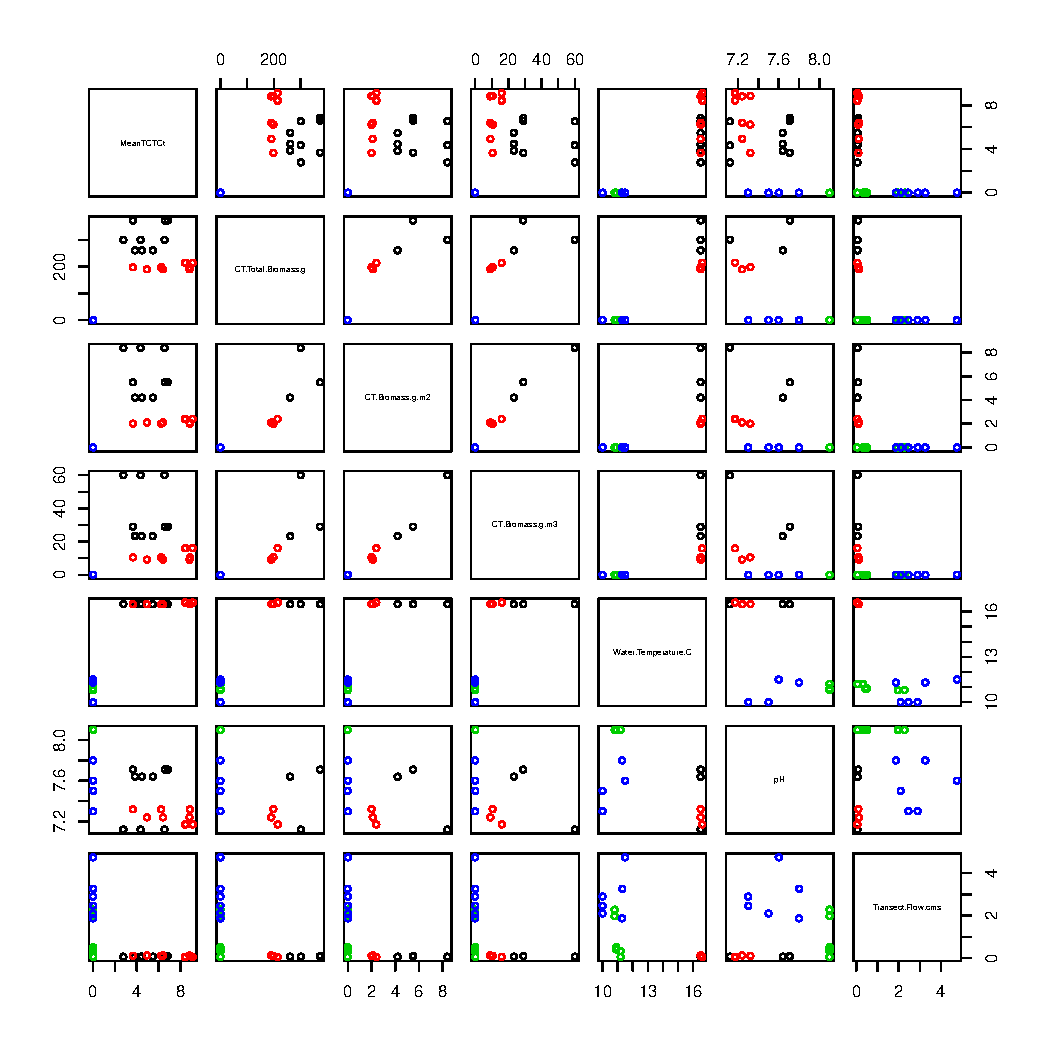
\includegraphics{AppendixImages/Ctpairs.pdf}
\caption{ \hspace{1mm}    Pairs plots for Cutthroat Trout. Black corresponds to Stream AAA, red corresponds to Stream BBB, green corresponds to Stream CCC and blue corresponds to Stream DDD.}
\label{fig:pairct}
\end{figure}



\begin{figure}[H]
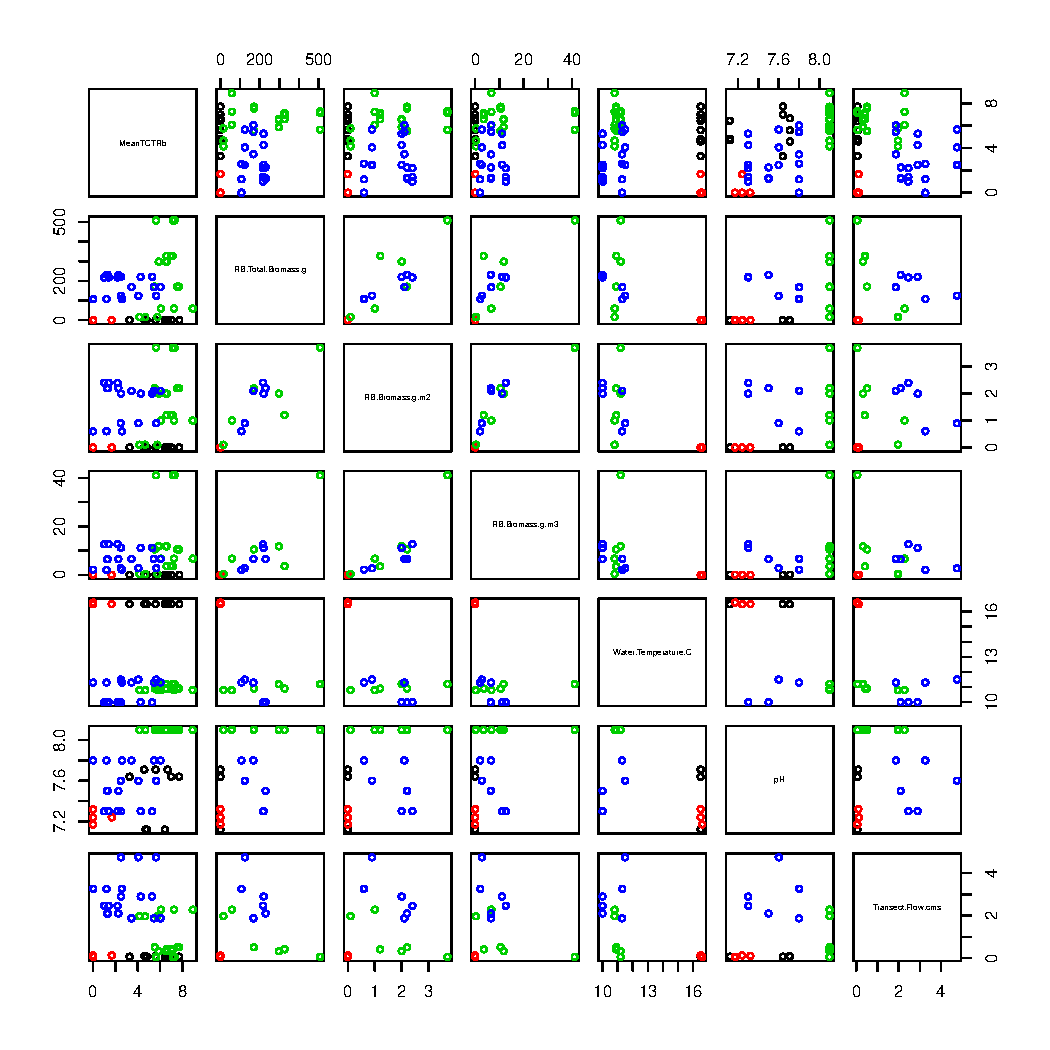
\includegraphics{AppendixImages/Rbpairs.pdf}
\caption{ \hspace{1mm}   Pairs plots for Rainbow Trout. Black corresponds to Stream AAA, red corresponds to Stream BBB, green corresponds to Stream CCC and blue corresponds to Stream DDD.}
\label{fig:pairrb}
\end{figure}



\section{Field Models}



\begin{figure}[H]
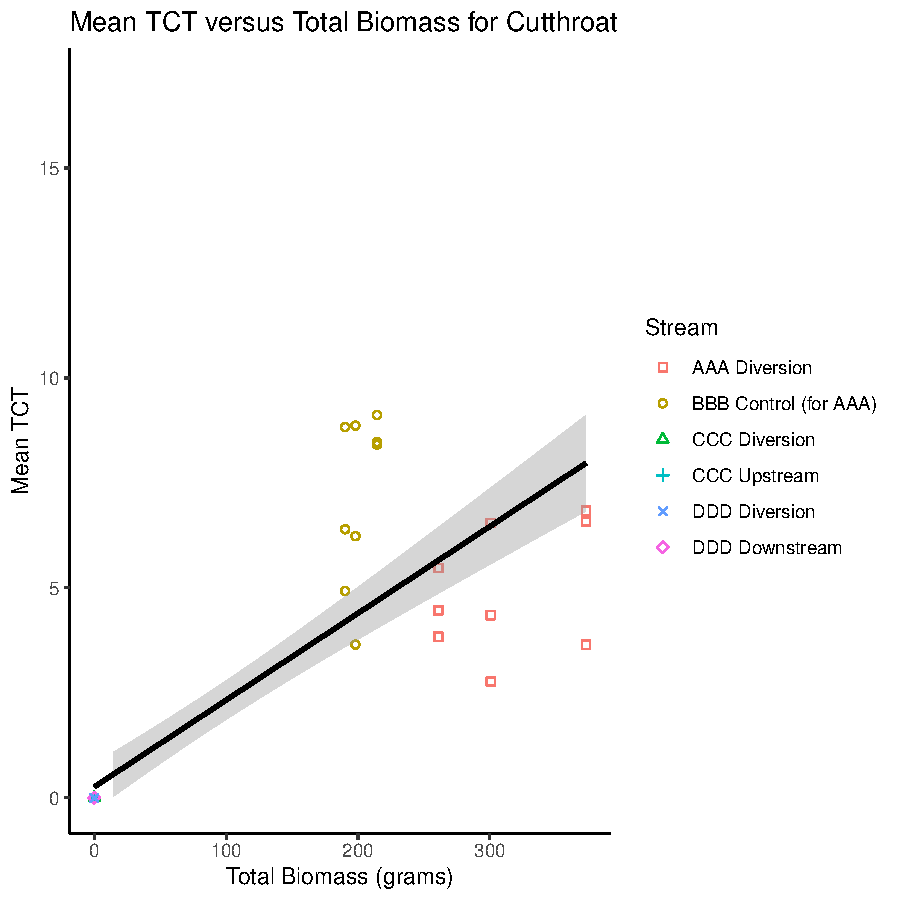
\includegraphics{AppendixImages/model_CT.pdf}
\caption{  \hspace{1mm}  Mean TCT versus Total Biomass for Cutthroat Trout. Included is the simple linear regression model and the 95\% Confidence limits for the regression line.}
\label{fig:ctanalysis}
\end{figure}



\begin{figure}[H]
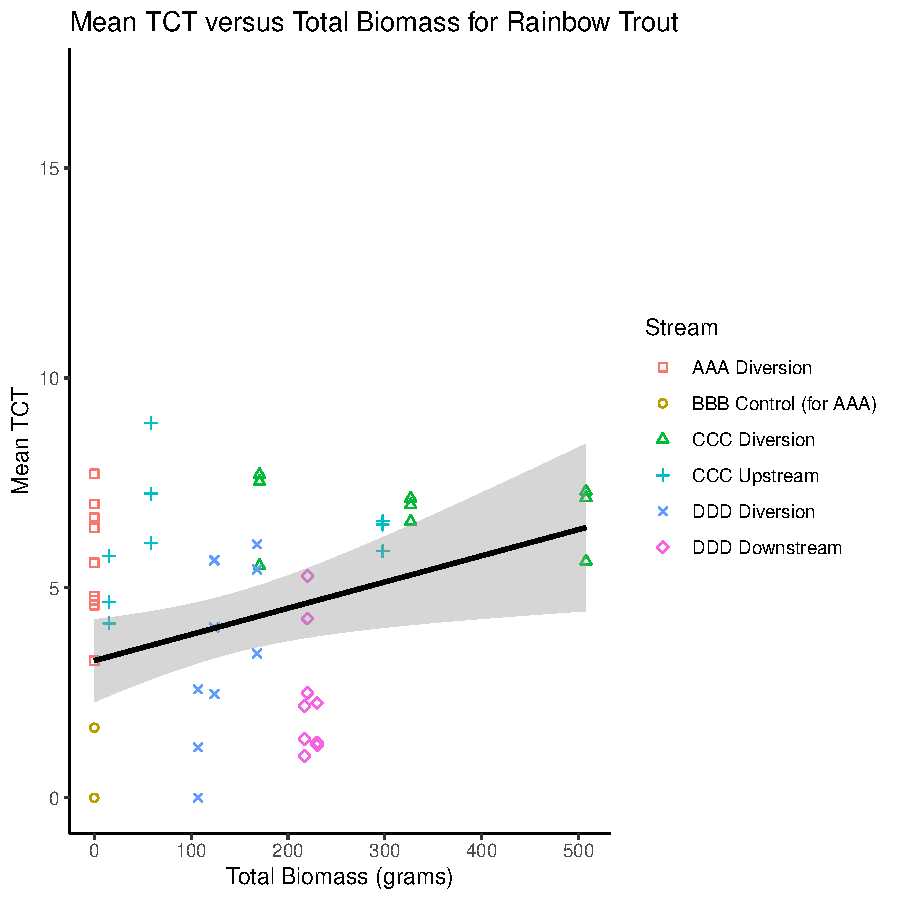
\includegraphics{AppendixImages/model_RB.pdf}
\caption{  \hspace{1mm} Mean TCT versus Total Biomass for Rainbow Trout. Included is the simple linear regression model and the 95\% Confidence limits for the regression line.}
\label{fig:rbanalysis}
\end{figure}






\begin{table}
 \begin{singlespace*}
\verbatiminput{AppendixImages/model_ct.txt}
\caption{\hspace{1mm}Model: model.ct}
\label{fig:mdct32}
\end{singlespace*}

\end{table}

Table~\ref{fig:mdct32} is the simple linear model for Cutthroat Trout (model.ct), our model achieves an $R^{2}$ of 0.716.



\begin{table}[H]
 \begin{singlespace*}
\verbatiminput{AppendixImages/model_rb.txt}
\caption{\hspace{1mm}Model: model.rb}
\label{fig:mdrb22}
\end{singlespace*}
\end{table}

Table~\ref{fig:mdrb22} summarizes the model that only considers Biomass for Rainbow Trout and it does not generalize well. The $R^{2}$ for this model is only 0.108. This implies that only considering the biomass of Rainbow Trout does not explain most of the variation in the data.





\section{Stepwise Elimination and Model Averaging}


\begin{table}[H]
 \begin{singlespace*}
\verbatiminput{AppendixImages/model_ef_step.txt}
\caption{\hspace{1mm}Backward elimination for all Fish.}
\label{fig:mafish1}
\end{singlespace*}
\end{table}



Table~\ref{fig:mafish1} summarizes backward stepwise elimination for all Fish, backward selection results in an $R^{2}$ of 0.171.



\begin{table}[H]
 \begin{singlespace*}
\verbatiminput{AppendixImages/model_ct_step.txt}
\caption{\hspace{1mm}Backward elimination for Cutthroat Trout.}
\label{fig:mdct32}
\end{singlespace*}
\end{table}



For Cutthroat, backwards stepwise elimination results in a model with an $R^{2}$ of 0.893.




\begin{table}[H]
 \begin{singlespace*}
\verbatiminput{AppendixImages/model_rb_step.txt}
\caption{\hspace{1mm}Backward elimination for Rainbow Trout.}
\label{fig:mdct32}
\end{singlespace*}
\end{table}


For Rainbow Trout, backward elimination results in a model with an $R^{2}$ of 0.605.






\begin{table}[H]
\begin{singlespace*}
\fontsize{11pt}{12pt}\selectfont
\verbatiminput{AppendixImages/modelavg_fish.txt}
\caption{\hspace{1mm}Model Averging for all Fish.}
\label{fig:mdct32}
\end{singlespace*}
\end{table}



  
\begin{table}[H]
\begin{singlespace*}
\fontsize{11pt}{12pt}\selectfont
\verbatiminput{AppendixImages/modelavg_ct.txt}
\caption{\hspace{1mm}Model Averaging for Cutthroat Trout.}
\label{fig:mdct3222}
\end{singlespace*}
\end{table}



\begin{table}[H]
\begin{singlespace*}
\fontsize{11pt}{12pt}\selectfont
\verbatiminput{AppendixImages/modelavg_rb.txt}
\caption{\hspace{1mm}Model Averaging for Rainbow Trout.}
\label{fig:mdct3412}
\end{singlespace*}
\end{table}


